\documentclass[../differential_geometry.tex]{subfiles}
\begin{document}
\section{Aula 07 - de Fevereiro, 2026}
\subsection{Motivações}
\begin{itemize}
	\item Análise no \(\mathbb{R}^{n}\).
\end{itemize}
\subsection{Análise no Espaço Euclidiano n-Dimensional}
A aula de hoje tem um propósito de nivelar o conhecimento dos alunos sobre análise no \(\mathbb{R}^{n}\), o conjunto de n-uplas de elementos reais,
\[
	\mathbb{R}^{n}=\{(x_1, x_2, \dotsc , x_{n}):\; x_{i}\in \mathbb{R},\; i=1,\dotsc ,n\}
\]
podendo ser vista como uma revisão àqueles que já sabem e uma introdução àqueles que não.
\begin{def*}
	A \textbf{bola aberta de centro a e raio \(\mathbf{r>0}\)} é o conjunto
	\[
		B(a, r)=\{x\in \mathbb{R}^{n}:\; \Vert x-a \Vert<r\}.\; \square
	\]
\end{def*}
\begin{def*}
	A \textbf{norma euclidiana} em \(\mathbb{R}^{n}\) é a norma \(\Vert \cdot  \Vert:\mathbb{R}^{n}\rightarrow \mathbb{R}\) dada por
	\[
		\Vert x \Vert = \sqrt[]{x_{1}^{2}+\dotsc +x_{n}^{2}}, \quad x=(x_1, \dotsc , x_{n}),
	\]
	e a \textbf{métrica usual}, ou a distância entre dois elementos \(x=(x_1,\dotsc ,x_{n})\) e \(a=(a_1,\dotsc ,a_{n})\), é definida como
	\[
		d(x, a)=\Vert x-a \Vert = \sqrt[]{(x_1-a_1)^{2}+\dotsc +(x_{n}-a_{n})^{2}}. \; \square
	\]
\end{def*}
Com as noções acima, fica fácil ver que
\[
	x\in B(a, r) \Longleftrightarrow (x_1-a_1)^{2}+\dotsc +(x_{n}-a_{n})^{2}<r^{2}.
\]
\begin{def*}
	Um subconjunto \(U\subseteq \mathbb{R}^{n}\) é dito \textbf{aberto} se, para todo elemento a em U, existe um \(r>0\) tal que
	\[
		B(a, r)\subseteq U. \; \square
	\]
\end{def*}
\begin{figure}[H]
	\begin{center}
		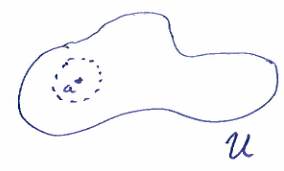
\includegraphics[height=0.6\textheight, width=0.6\textwidth, keepaspectratio]{./Images/open_set_07.png}
	\end{center}
\end{figure}

\begin{example}
	\begin{itemize}
		\item[1)] A bola aberto \(B(a, r)\) é um subconjunto aberto de \(\mathbb{R}^{n}\);
		\item[2)] Uma a célula/caixa, dada por
		      \[
			      (a_1, b_1)\times (a_2, b_2)\times \dotsc \times (a_{n}, b_{n}), \quad a_{i}<b_{i},\; i=1,\dotsc ,n,
		      \]
		      é um subconjunto aberto de \(\mathbb{R}^{n}\);
		\item[3)] O próprio \(\mathbb{R}^{n}\) é aberto; e
		\item[4)] O conjunto vazio \(\emptyset \) é um aberto.
	\end{itemize}
\end{example}

Seja U um aberto de \(\mathbb{R}^{n}\) e \(f:U\rightarrow \mathbb{R}^{n}\) uma aplicação dada por
\[
	f(u)=f(u_1,\dotsc ,u_{n})=(f^{1}(u_1,\dotsc ,u_{n}), f^{2}(u_1,\dotsc , u_{n}), \dotsc , f^{m}(u_1,\dotsc ,u_{n})),
\]
onde u é um elemento de U e (\textbf{ATENÇÃO!}) estamos utilizando a notação de superíndice para as coordenadas de uma função multivariada: \(f^{k}(u_1,\dotsc , u_{n})\) não é a k-ésima potência de f, mas sim a k-ésima coordenada!
\begin{def*}
	Uma aplicação f é \textbf{suave} (ou seja, \(\mathcal{C}^{\infty}\)), se as derivadas parciais das funções \(f^{i},\; i=1,\dotsc ,n\), existem em todas as ordens e são todas contínuas. \(\square\)
\end{def*}
\begin{example}
	As aplicações
	\begin{align*}
		 & f:\mathbb{R}^{2}\rightarrow \mathbb{R}^{3},\; f(u_1, u_2)=(u_1, u_2, \overbrace{u_{1}^{2}+u_{2}^{2}}^{\mathclap{\text{Aqui é potência! Atenção ao contexto}}}) \\
		 & f:B(0,1)\subseteq \mathbb{R}^{2}\rightarrow \mathbb{R}^{3},\; f(u_1, u_2)=(u_1, u_2, \sqrt[]{1-u_{1}^{2}-u_{2}^{2}})
	\end{align*}
	são ambas suaves.
\end{example}

\begin{def*}
	Seja \(f=(f^{1},\dotsc, f^{m}):U\subseteq \mathbb{R}^{n}\rightarrow \mathbb{R}^{m}\) uma aplicação suave, onde U é um aberto de \(\mathbb{R}^{n}\), e tome um ponto p em U. A \textbf{matriz jacobiana de f em p} é a matriz das derivadas de cada coordenada, com respeito a cada variável:
	\[
		J_{p}(f)=\begin{pmatrix}
			\frac{\partial^{}f^{1}}{\partial u_{1}^{}}(p) & \dotsc & \frac{\partial^{}f^{1}}{\partial u_{n}^{}}(p) \\
			\frac{\partial^{}f^{2}}{\partial u_{1}^{}}(p) & \dotsc & \frac{\partial^{}f^{2}}{\partial u_{n}^{}}(p) \\
			\vdots                                        & \ddots & \vdots                                        \\
			\frac{\partial^{}f^{m}}{\partial u_{1}^{}}(p) & \dotsc & \frac{\partial^{}f^{m}}{\partial u_{n}^{}}(p)
		\end{pmatrix},
	\]
	e a aplicação linear \(\mathrm{d}f_{p}:\mathbb{R}^{n}\rightarrow \mathbb{R}^{m}\) definida por
	\[
		\mathrm{d}f_{p}(h)=J_{p}(f)\cdot h
	\]
	é a \textbf{derivada de f no ponto p e direção h}. \(\square\)
\end{def*}
Como a aplicação \(\mathrm{d}f_{p}\) é uma aplicação linear, a sua imagem \(\mathrm{d}f_{p}(\mathbb{R}^{n})\) é um subespaço vetorial de \(\mathbb{R}^{m}\), especificamente o subespaço gerado por seu valor em cada elemento da base de seu domínio:
\[
	\mathrm{d}f_{p}(\mathbb{R}^{n})=\mathrm{span}\{\mathrm{d}f_{p}(e_1), \dotsc , \mathrm{d}f_{p}(e_{n})\},
\]
onde \(\{e_1,\dotsc , e_{n}\}\) é a base canônica de \(\mathbb{R}^{n}\). Assim, como para cada i entre 1 e n, a derivada de f no ponto p em direção a \(e_{i}\) é dada por
\[
	\mathrm{d}f_{p}(e_{i})=\begin{pmatrix}
		\frac{\partial^{}f^{1}}{\partial u_{1}^{}}(p) & \dotsc & \frac{\partial^{}f^{1}}{\partial u_{n}^{}}(p) \\
		\frac{\partial^{}f^{2}}{\partial u_{1}^{}}(p) & \dotsc & \frac{\partial^{}f^{2}}{\partial u_{n}^{}}(p) \\
		\vdots                                        & \ddots & \vdots                                        \\
		\frac{\partial^{}f^{m}}{\partial u_{1}^{}}(p) & \dotsc & \frac{\partial^{}f^{m}}{\partial u_{n}^{}}(p)
	\end{pmatrix} \begin{pmatrix}
		0      \\
		\vdots \\
		1      \\
		0      \\
		\vdots \\
		0
	\end{pmatrix},
\]
segue que
\[
	\mathrm{d}f_{p}(e_{i}) = \biggl(\frac{\partial^{}f^{1}}{\partial u_{i}^{}}(p), \dotsc , \frac{\partial^{}f^{m}}{\partial u_{i}^{}}(p)\biggr) = \frac{\partial^{}f}{\partial u_{i}^{}}(p).
\]
Logo, o subespaço vetorial \(\mathrm{d}f_{p}(\mathbb{R}^{n})\) é gerado pelas colunas da matriz de Jordan:
\[
	\mathrm{d}f_{p}(\mathbb{R}^{n})=\biggl\{\frac{\partial^{}f}{\partial u_1^{}}(p), \dotsc , \frac{\partial^{}f}{\partial u_{n}^{}}(p)\biggr\}.
\]
\begin{example}
	\begin{itemize}
		\item[1)] Considere uma aplicação \(f:\mathbb{R}^{n}\rightarrow \mathbb{R}\); então, \(\mathrm{d}f_{p}:\mathbb{R}^{n}\rightarrow \mathbb{R}\), e é dada por
		      \[
			      \mathrm{d}f_{p}(h)=J_{p}(f)\cdot h= \nabla_{p}f \cdot h = \biggl(\frac{\partial^{}f}{\partial u_1^{}}(p),\dotsc , \frac{\partial^{}f}{\partial u_{n}^{}}(p)\biggr) \begin{pmatrix}
				      h_1    \\
				      \vdots \\
				      h_{2}
			      \end{pmatrix}.
		      \]
		      Daí, como \(\mathrm{d}f_{p}(\mathbb{R}^{n})\) será um subespaço vetorial de \(\mathbb{R}\), os únicos casos possíveis são \(\mathrm{d}f_{p}(\mathbb{R}^{n})=\mathbb{R}\) ou
		      \[
			      \mathrm{d}f_{p}(\mathbb{R}^{n})=\{0\} \Longleftrightarrow  \nabla_{p}f=(0,0,\dotsc ,0).
		      \]
		\item[2)] Agora, vamos considerar \(f:\mathbb{R}^{2}\rightarrow \mathbb{R}^{3}\) a aplicação \(f(u, v)=(u, v, u^{2}+v^{2})\); então, no ponto \(p=(u, v)\), teremos
		      \[
			      J_{p}f=\begin{bmatrix}
				      1  & 0  \\
				      0  & 1  \\
				      2u & 2v
			      \end{bmatrix} \Rightarrow \mathrm{d}f_{p}(\mathbb{R}^{2})= \mathbb{R} \cdot \biggl\{\begin{pmatrix}
				      1 \\
				      0 \\
				      2u
			      \end{pmatrix}, \begin{pmatrix}
				      0 \\
				      1 \\
				      2v
			      \end{pmatrix}\biggr\},
		      \]
		      um subespaço de dimensão 2 para qualquer p em \(\mathbb{R}^{2}\).
		\item[3)] Seja \(f:\mathbb{R}^{2}\rightarrow \mathbb{R}^{3}\) a aplicação \(f(u, v)=(u, v^{2}, uv)\). Sua jacobiana em p é
		      \[
			      J_{p}f=\begin{pmatrix}
				      1 & 0  \\
				      0 & 2v \\
				      v & u
			      \end{pmatrix},
		      \]
		      de modo que sua imagem é
		      \[
			      \mathrm{d}f_{p}(\mathbb{R}^{2})=\mathbb{R}\cdot \biggl\{\begin{pmatrix}
				      1 \\
				      0 \\
				      v
			      \end{pmatrix}, \begin{pmatrix}
				      0  \\
				      2v \\
				      u
			      \end{pmatrix}\biggr\},
		      \]
		      mas a dimensão depende do valor de p:
		      \[
			      \mathrm{dim}(\mathrm{d}f_{p}(\mathbb{R}^{2})) = \left\{\begin{array}{ll}
				      2, & \quad p\neq (0,0) \\
				      1, & \quad p=(0,0)
			      \end{array}\right..
		      \]
		\item[4)] Para \(f:\mathbb{R}^{2}\rightarrow \mathbb{R}^{3},\; f(u, v)=(u^{2}, v^{2}, uv)\), temos
		      \[
			      J_{p}f=\begin{pmatrix}
				      2u & 0  \\
				      0  & 2v \\
				      v  & u
			      \end{pmatrix} \Rightarrow \mathrm{dim}(\mathrm{d}f_{p}(\mathbb{R}^{2})) = \left\{\begin{array}{ll}
				      2, & \quad p\neq (0,0) \\
				      0, & \quad p=(0,0)
			      \end{array}\right..
		      \]
	\end{itemize}
\end{example}
\subsection{Regra da Cadeia e Função Implícita}
Sejam \(f:U\subseteq \mathbb{R}^{n}\rightarrow \mathbb{R}^{m}\) e \(g:V\subseteq \mathbb{R}^{m}\rightarrow \mathbb{R}^{p}\), onde U é um aberto de \(\mathbb{R}^{n}\) e V de \(\mathbb{R}^{m}\), duas aplicações suaves; considere a aplicação composta \(g\circ f:f^{-1}(V)\rightarrow \mathbb{R}^{p}\).
\begin{figure}[H]
	\begin{center}
		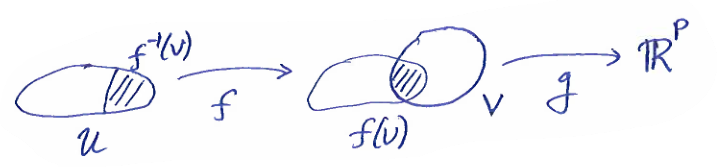
\includegraphics[height=0.9\textheight, width=0.9\textwidth, keepaspectratio]{./Images/chain_rule_07.png}
	\end{center}
\end{figure}
Então, temos a regra de composição
\[
	\mathrm{d}(g\circ f)_{p} = (\mathrm{d}g)_{f(p)} \circ \mathrm{d}f_{p},
\]
que é a versão generalizada da \hypertarget{chain_rule}{\textbf{regra da cadeia}}! Em particular, no caso em que \(n=m\), a matriz jacobiana vira uma matriz quadrada, e se \(\det{(J_{p}(f))}\) for não nulo, então
\[
	\mathrm{d}f_{p} :\mathbb{R}^{n}\rightarrow \mathbb{R}^{n}
\]
é um isomorfismo.
\begin{def*}
	Sejam U e V dois abertos de \(\mathbb{R}^{n}\). Uma aplicação \(f:U\rightarrow V\) é um \textbf{difeomorfismo} se:
	\begin{itemize}
		\item[i)] f é bijetora; e
		\item[ii)] Tanto f quanto \(f^{-1}\) são suaves. \(\square\)
	\end{itemize}
\end{def*}
\hypertarget{inverse_function}{
	\begin{theorem*}[Teorema da Função Inversa]
		Seja \(f:U\subseteq \mathbb{R}^{n}\rightarrow \mathbb{R}^{n}\) uma aplicação suave, onde U é um aberto. Suponha que \(\mathrm{d}f_{p}\) é um isomorfismo no ponto p de U; então, existe um aberto V de \(\mathbb{R}^{n}\) tal que:
		\begin{itemize}
			\item[1)] \(p\in V \subseteq U\);
			\item[2)] \(f(V)\) é um aberto; e
			\item[3)] \(f:V\rightarrow f(V)\) é um difeomorfismo.
		\end{itemize}
	\end{theorem*}
}
\hypertarget{implicit_function}{
	\begin{theorem*}[Teorema da Função Implícita]
		Seja \(f:U\subseteq \mathbb{R}^{p+m}\rightarrow \mathbb{R}^{m}\) uma aplicação suave, onde U é um aberto. Denote por \((u_{1},\dotsc , u_{p}, v_1, \dotsc , v_{m})\) as coordenadas de \(\mathbb{R}^{p+m}\) e considere a matriz \(m\times m\) dada por
		\[
			\begin{pmatrix}
				\frac{\partial^{}f^{1}}{\partial v_1^{}}   & \dotsc & \frac{\partial^{}f^{1}}{\partial v_{m}^{}} \\
				\frac{\partial^{}f^{2}}{\partial v_1^{}}   & \dotsc & \frac{\partial^{}f^{2}}{\partial v_{m}^{}} \\
				\vdots                                     & \ddots & \vdots                                     \\
				\frac{\partial^{}f^{m}}{\partial v_{1}^{}} & \dotsc & \frac{\partial^{}f^{m}}{\partial v_{m}^{}}
			\end{pmatrix}.
		\]
		Se essa matriz tem determinante não nulo em um ponto \((a, b)\) de U, então existem abertos V de \(\mathbb{R}^{p}\) que contém a; \(W\subseteq \mathbb{R}^{m}\) que contém b; e uma aplicação suave \(g:V\rightarrow W\), tais que:
		\[
			(u,v)\in V\times W\subseteq U,\; f(u, v)=c \Longleftrightarrow v = g(u),
		\]
		ou seja, o conjunto de nível \(f = c\) (\(=f(a, b)\)) é o gráfico da aplicação g.
	\end{theorem*}
}
\begin{figure}[H]
	\begin{center}
		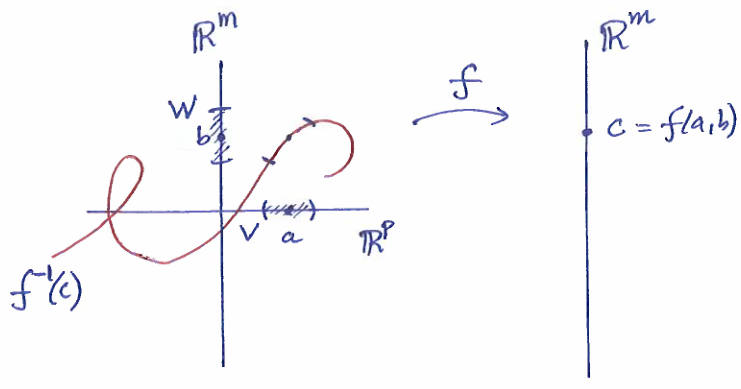
\includegraphics[height=0.8\textheight, width=0.8\textwidth, keepaspectratio]{./Images/implicit_function_07.png}
	\end{center}
\end{figure}
\end{document}

